\documentclass{mwart}
\usepackage{multicol}
\usepackage{polski} % Pozwala na użycie polskiego. Ustawia między innymi fontenc na T1
\usepackage[utf8]{inputenc} % Informuje o kodowaniu
\usepackage{enumitem}
\usepackage{xcolor}
\usepackage{xcolor}% http://ctan.org/pkg/xcolor
\usepackage{hyperref}
\usepackage{listings}
\usepackage{float} % Ustawianie obrazów
\usepackage[caption = false]{subfig} % Wiele obrazów w jednej figurze
\definecolor{LinkColor}{HTML}{1d5cc1}
\renewcommand{\labelitemi}{\textbullet} % Zmiana symbolu wliczeń

\lstset{
  basicstyle=\ttfamily,
  columns=fullflexible,
  breaklines=true,
  postbreak=\mbox{\textcolor{red}{$\hookrightarrow$}\space},
}

\definecolor{LinkColor}{HTML}{1d5cc1}

\usepackage{tabto}

\usepackage{graphicx} % Pakiet do obrazów
\graphicspath{ {./Obrazy/} } % Folder, z którego będą brane obrazy

% Nie twórz nowych stron
\usepackage{etoolbox}
\makeatletter
% \patchcmd{\chapter}{\if@openright\cleardoublepage\else\clearpage\fi}{}{}{}
\makeatother

\newcommand{\paragraphnl}[1]{\paragraph{#1} \mbox{} \\} % Paragraf z nową linią

\title{PRIR Sprawozdanie końcowe -- Gra w życie}
\author{Krzysztof Dąbrowski 293101}
\date{\today}

\begin{document}
\maketitle{}

\tableofcontents{}

\section{Opis projektu}
W ramach projektu został zmodyfikowany symulator automatów komórkowych \textit{Wireworld} i \textit{Gra w życie} napisany oryginalnie w ramach przedmiotu \texttt{JIMP2}. Przyjęta forma zadania pozwoliła na rozwój umiejętności związanych z utrzymaniem kodu. Rozbudowa projektu o zrównoleglenie obliczeń dobrze wpisuję się w typowe zastosowanie programowania równoległego, które często nie zmienia funkcjonalności programu, lecz pozwala przyśpieszyć zastosowane rozwiązania lub pośrednio umożliwić przetwarzanie większych zbiorów danych.

\section{Opis uruchomienia}
W celu łatwego uruchomienia i konfiguracji projektu zastosowany został system automatyzacji budowy projektu \textit{Gradle}. Został on skonfigurowany w ten sposób, że aplikację można łatwo uruchomić poniższym poleceniem. Przykład zakłada, że lokalizacja terminala jest ustawiona na katalog \textbf{zawierający projekt}.

\begin{lstlisting}[language=bash]
./gradlew run 
\end{lstlisting}

Dzięki zastosowaniu \textit{Gradle wrapper} nie jest wymagana instalacja narzędzia \textit{Gradle}.

\section{Modernizacja kodu}
Oryginalny kod był jednym z pierwszy moich projektów w języku Java. W celu uproszczenia rozwoju projektu oraz późniejszego korzystania z niego została przeprowadzona modernizacja zastosowanych technologii.

\subsection*{Biblioteki}
Początkowo projekt nie korzystał z narzędzia do budowy kodu a biblioteki były manualnie dołączane do ścieżki kompilatora. Podejście to zmienione na zastosowanie narzędzia \textit{Gradle}, które umożliwia automatyzację dołączania bibliotek oraz budowy aplikacji. Użyte biblioteki zostały również aktualizowane do nowych wersji.

\subsection*{Java 11}
Poziom języka został podniesiony z wersji 8 do 11. Umożliwiło to zastosowanie nowych funkcjonalności takich jak słowo kluczowe \texttt{var} oraz zastosowanie mechanizmu modułów.
Mechanizm modułów został wykorzystany głównie przy dołączaniu biblioteki \textit{Java FX}.

\subsection*{Struktura kodu}
Zmieniona została struktura modułów projektu, tak by była zgodna z panującymi standardami w większości projektów. Dodatkowo zasoby takie jak pliki \texttt{.fxml} zostały przeniesione do katalogu \texttt{resources}, co ułatwiło ich ładowanie.

\section{Projekt zrównoleglenia}
W celu zaprojektowania sposobu zrównoleglania programu zastosowana została metodyka PCAM. Poniżej przedstawione są wnioski wynikające z poszczególnych etapów.

\subsection{Dekompozycja}
Ponieważ do obliczenia stanów komórek kolejnego pokolenia wymagana jest informacja o ich stanie w aktualnym pokoleniu najlepiej jest zrównoleglić obliczanie stanów komórek nowego pokolenia.

Stan każdej komórki może być obliczony niezależnie, więc ziarnistość rozwiązania kształtuje się na poziomie pojedynczej komórki automatu.

Zastosowana została głównie dekompozycja domenowa.

\subsection{Komunikacja}
Komunikacja między wątkami nie jest wymagana. Każdy wątek może korzystać z pamięci współdzielonej w celu uzyskania informacji o stanie komórek z poprzedniego pokolenia.

\subsection{Scalanie}
Etap scalania został zrealizowany na różne sposoby w kolejnych wersjach projektu. Zmiana wersji scalania jest możliwa poprzez przejście na odpowiadającą gałąź systemu kontroli wersji \textit{git}.

Zastosowane metody scalania to
\begin{itemize}
  \item jedno zadanie dla każdej komórki
  \item stała wielkość komórek przypadających na poszczególne zadanie
  \item stała liczba zadań równa liczbie procesorów
\end{itemize}

\subsubsection{Odwzorowanie}
Odwzorowanie zadań na zasoby procesora jest realizowane automatycznie przez maszynę wirtualną Java. Pośrednio jest to kontrolowane przez tworzenie klas \texttt{Thread} lub wykorzystanie \texttt{ExecutorContext} z \textit{Concurrency API}.

\section{Implementacja zrównoleglenia}
Przy pisaniu projektu zostały zastosowane dwa API pozwalające na zrównoleglenie wykonania programu. Dzięki temu możliwe jest porównanie wydajności tych pojeść.

\subsection{Thread}
Pierwszym podejściem jest zastosowanie klas \texttt{Runnable} a następnie utworzenie na ich podstawie wątków \texttt{Thread}. Każdy wątek po utworzeniu zostanie utworzony. Następnie zostaną one dołączone do wątku głównego przy pomocy metody \texttt{join()}.

\subsection{Concurrency API}
Drugim podejściem zastosowanym w projekcie było skorzystanie z rozwiniętego w Javie 8 \textit{Concurrency API}. Realizuje ono abstrakcję na bezpośrednie wątki. Zamiast tego tworzone są \texttt{Executory} oraz zdania typu \texttt{Callable}. Następnie zdania są przekazywane do egzekutorów, w wyniku czego powstają obiekty \texttt{Future}. Po zakończeniu wykonania zadań możliwe jest odczytanie wyniku z obiektu \texttt{Future}.

W projekcie zastosowany został globalny \texttt{ExecutorService} typu \texttt{FixedThreadPool} z liczbą wątków równą liczbie dostępnych procesorów w systemie. Zaimplementowany na podstawie wzorca \textit{Singleton}.
Przy symulacji następnego pokolenia w zależności od zastosowanego odwzorowania tworzona jest odpowiednia lista zadań. Następnie jest ona realizowana przez globalny egzekutor.


\section{Analiza uzyskanych wyników}
W celu zbadania wydajności różnych podejść został napisany test wydajnościowy. Przeprowadza on określoną liczbę symulacji 50 pokoleń dla planszy o wymiarach 1000 na 1000. Celowo wybrana została plansza o dużych rozmiarach.

Wyniki uzyskanie w różnych podejściach zostały przeanalizowane przy pomocy narzędzi z bibliotek Pandas i Plotly do języka Python.

\subsection{Podejście sekwencyjne}
Zbadanie wydajności bez zrównoleglenia.

\paragraph{Średni czas symulacji: } 1868.68 ms

\begin{figure}[H]
  \centering
  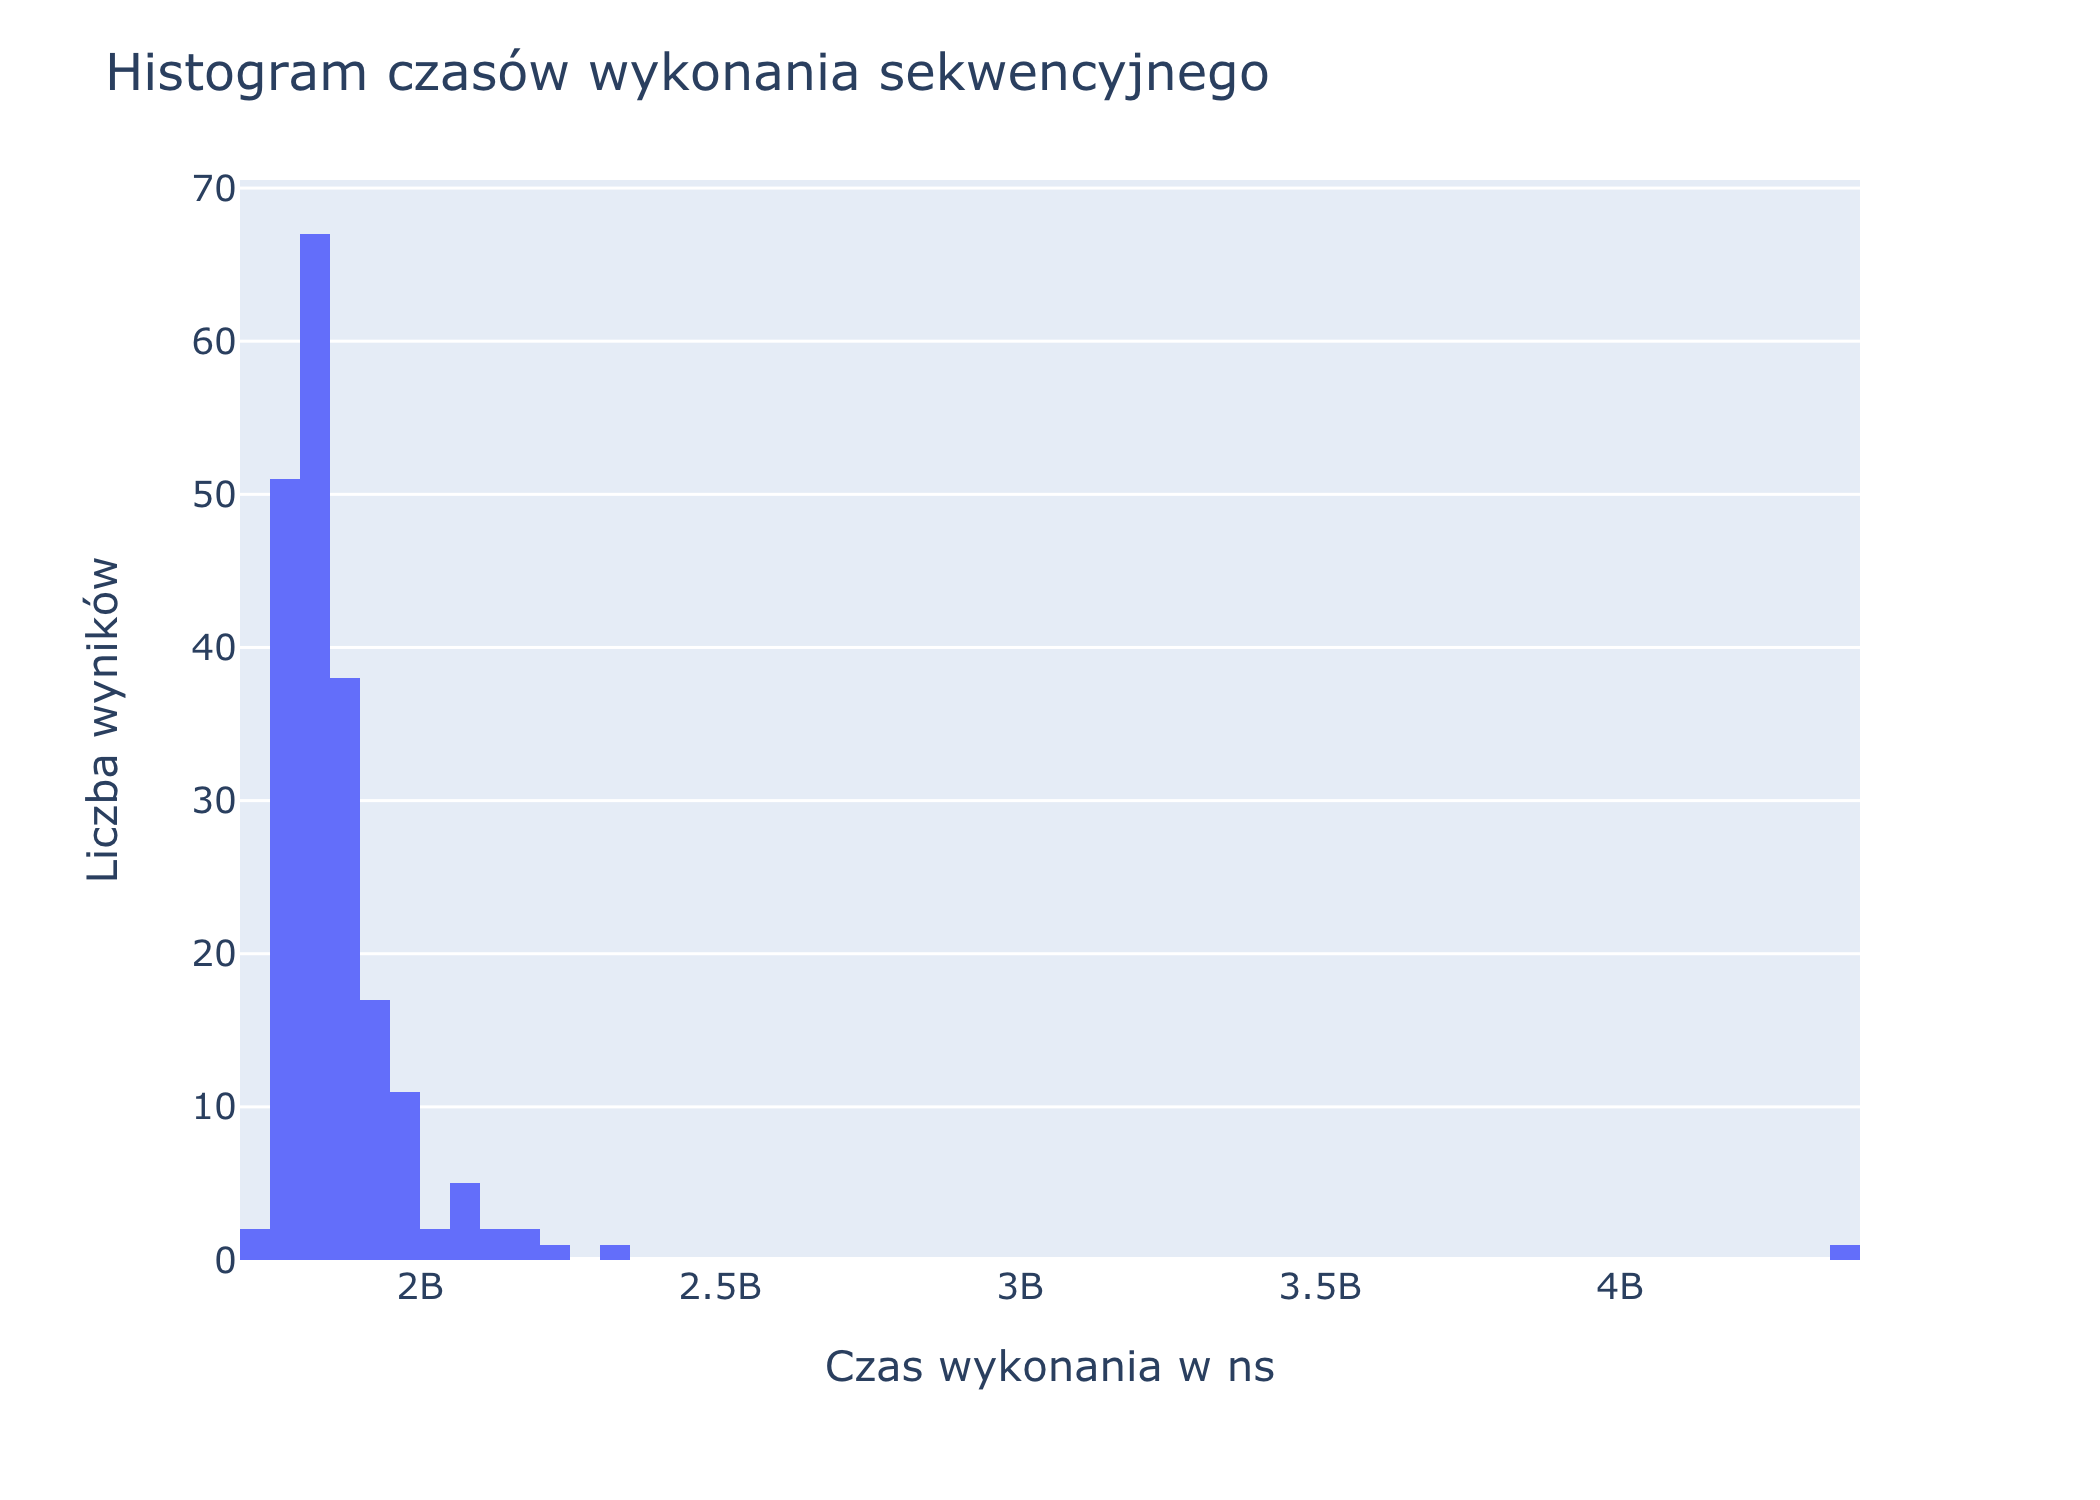
\includegraphics[width=0.9\textwidth]{Sequential_histogram}
  \caption{Histogram czasów wykonania sekwencyjnego}
\end{figure}

\subsection{Concurrency API}
Zbadanie wydajności programu przy zastosowaniu klas \texttt{Future} i \texttt{Executor}.

\subsubsection{Future dla każdej komórki}
\paragraph{Średni czas symulacji: } 19156.33 ms


\begin{figure}[H]
  \centering
  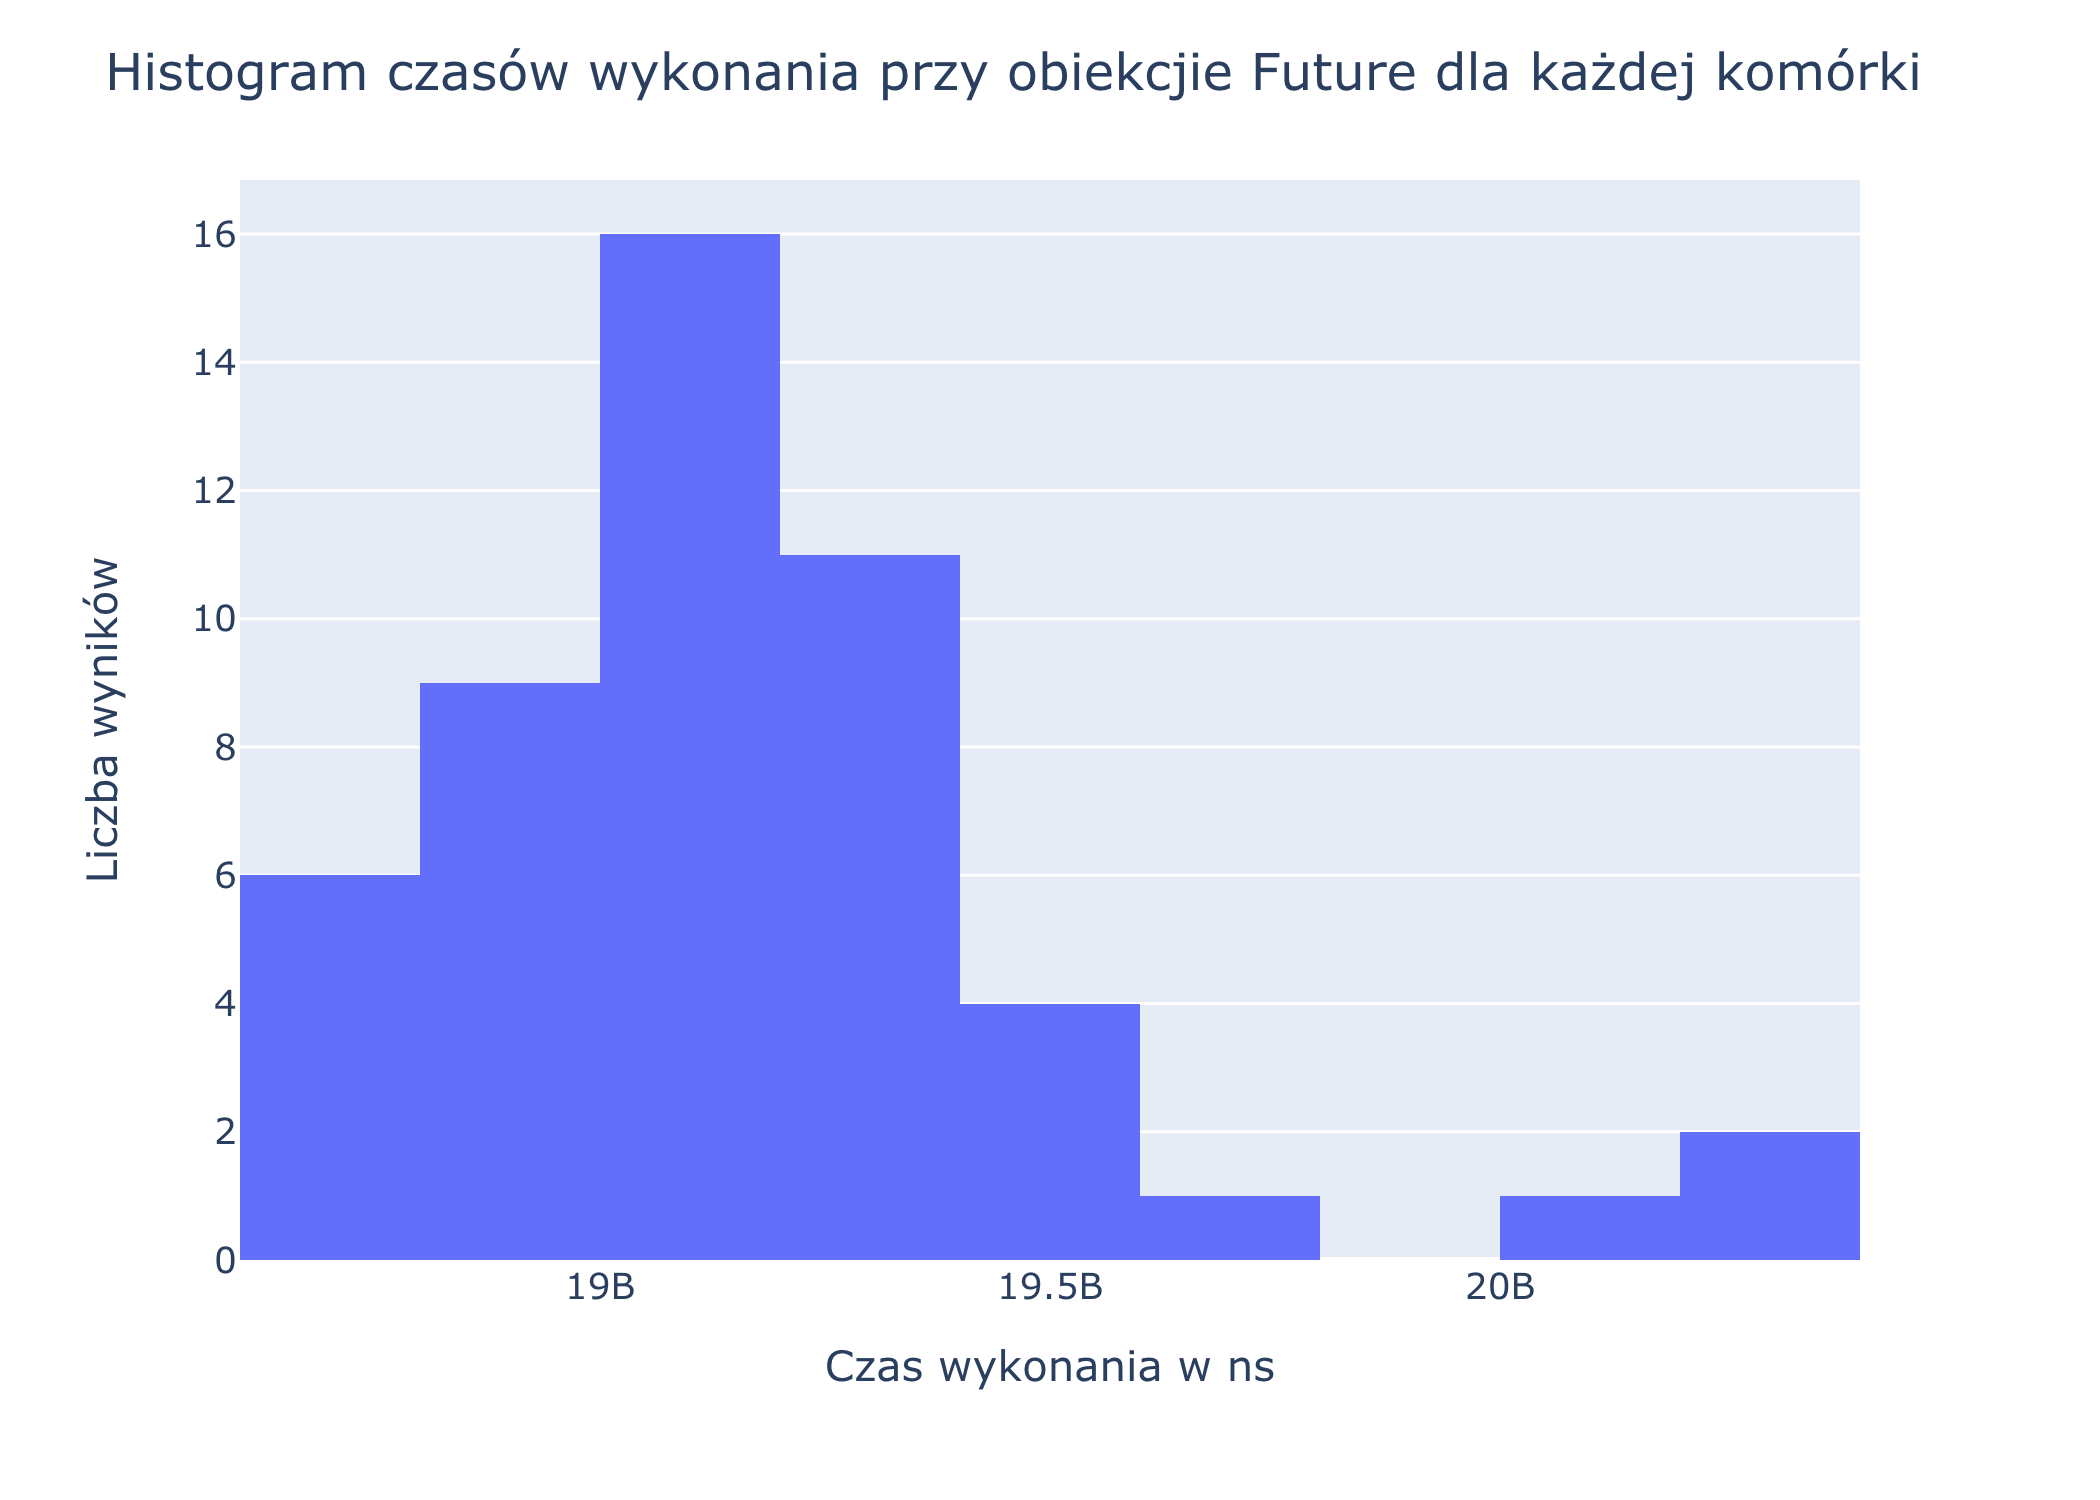
\includegraphics[width=0.9\textwidth]{Parallel_Future_for_each_cell_game_of_life_performance}
  \caption{Histogram czasów wykonania przy obiekcie Future dla każdej komórki}
\end{figure}

\subsubsection{Stała wielkość 200 komórek na Future}
\paragraph{Średni czas symulacji: } 653.89 ms


\begin{figure}[H]
  \centering
  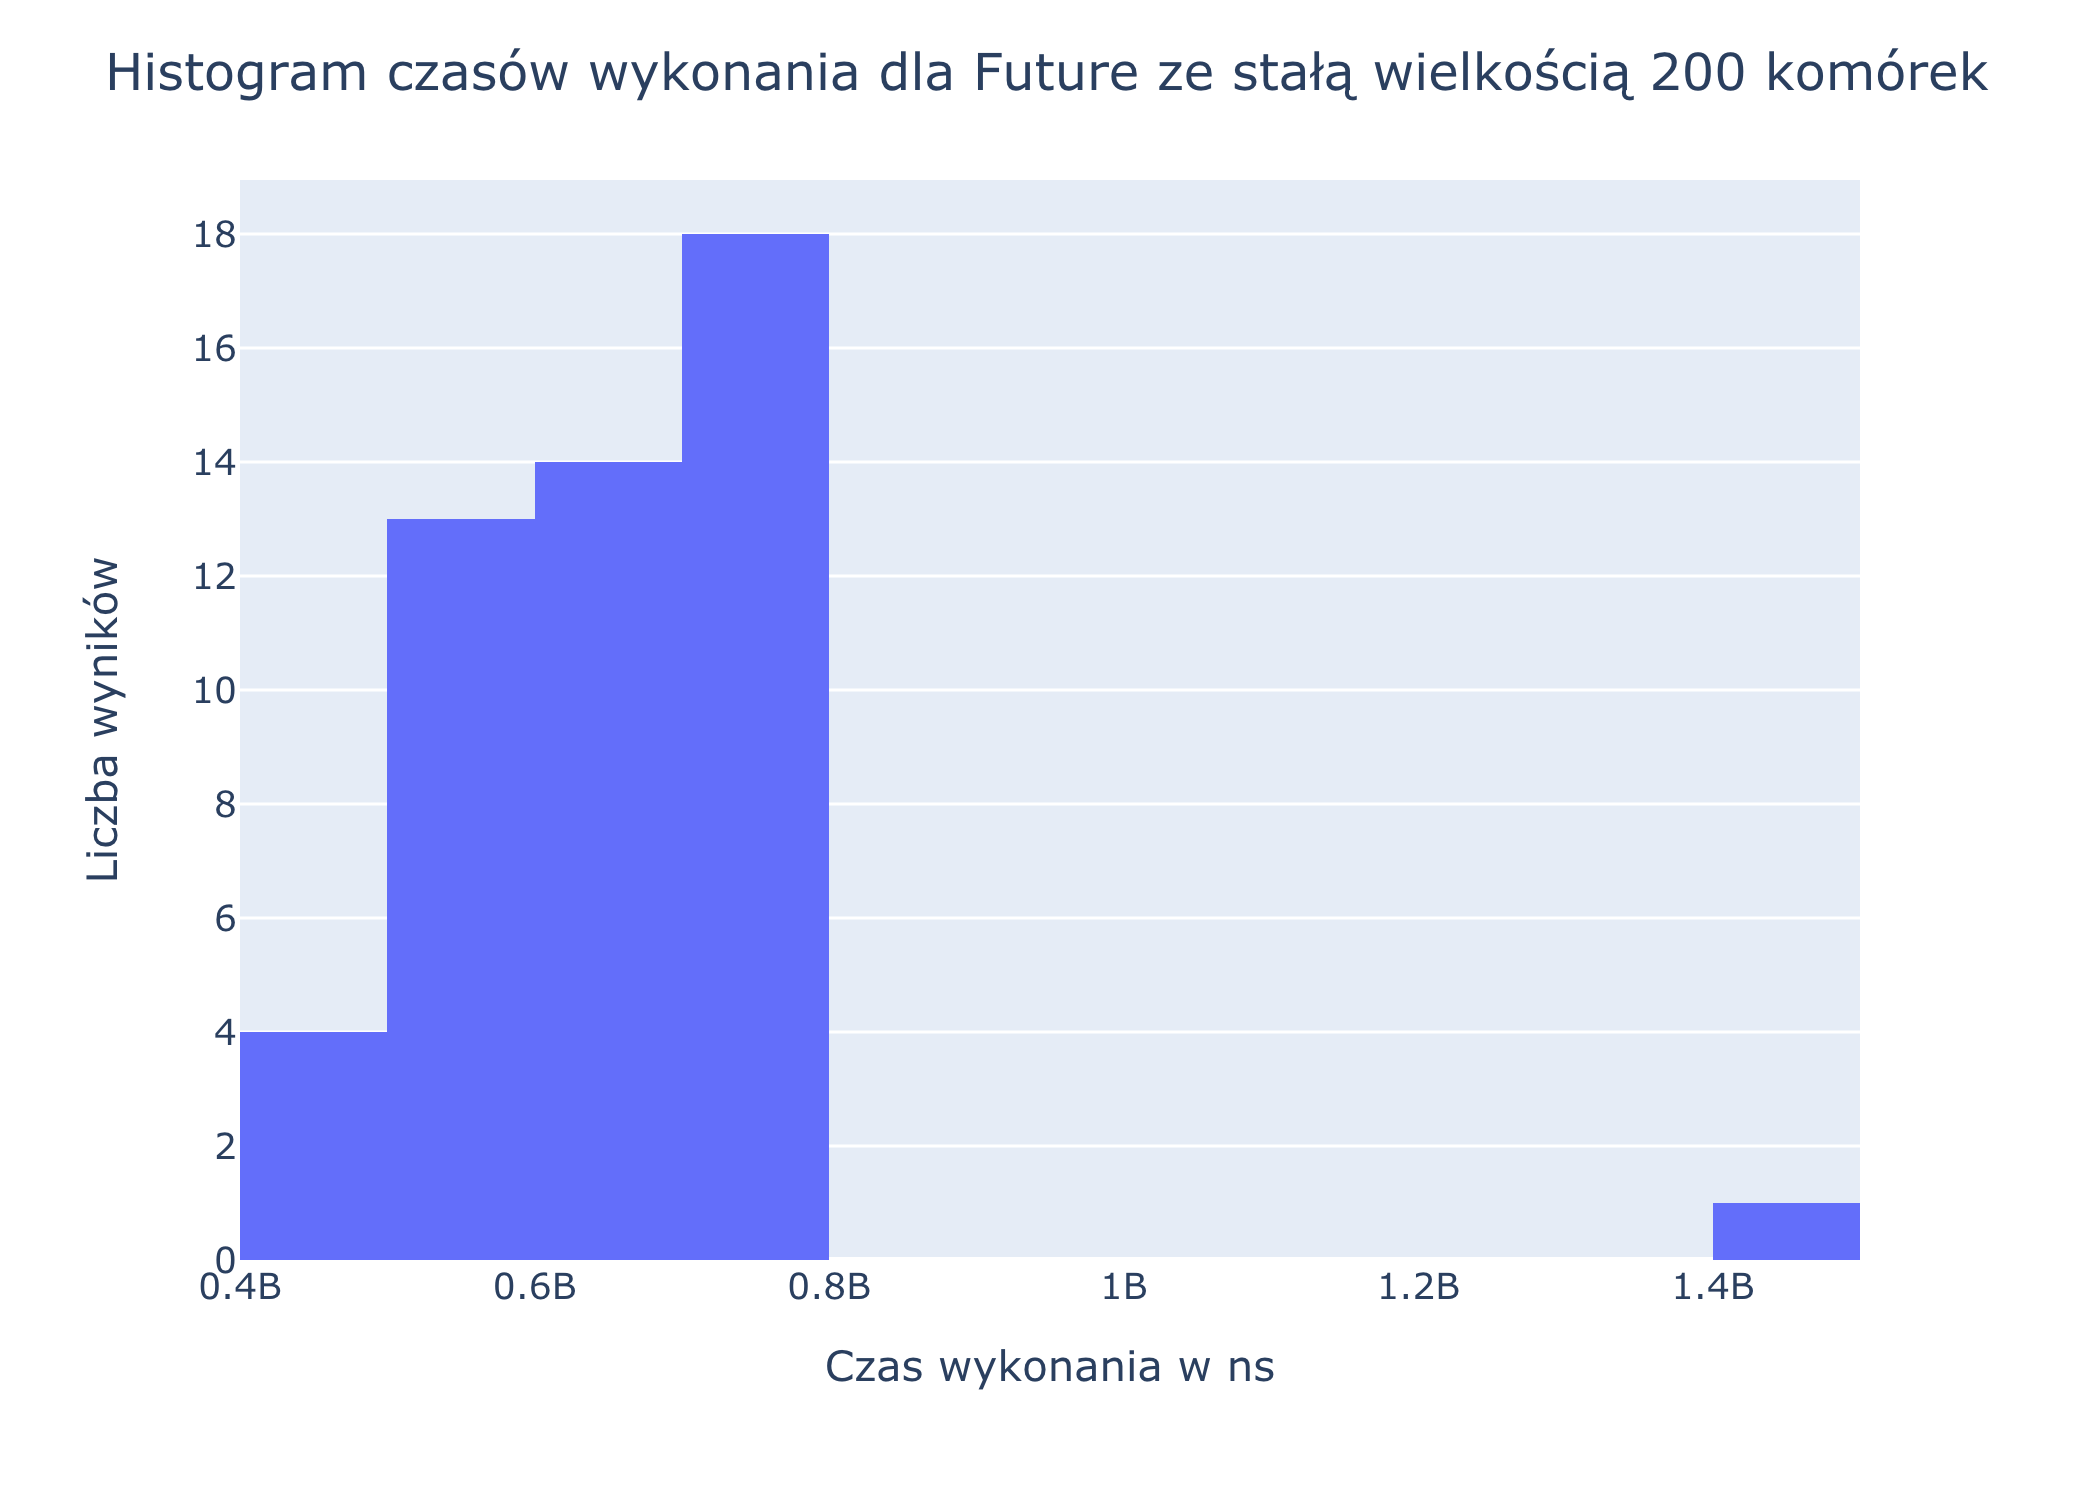
\includegraphics[width=0.9\textwidth]{Parallel_Future_fix_chunk_200_game_of_life_performance}
  \caption{Histogram czasów wykonania dla Future ze stałą wielkością 200 komórek}
\end{figure}

\subsubsection{Stała wielkość 500 komórek na Future}
\paragraph{Średni czas symulacji: } 724.56 ms


\begin{figure}[H]
  \centering
  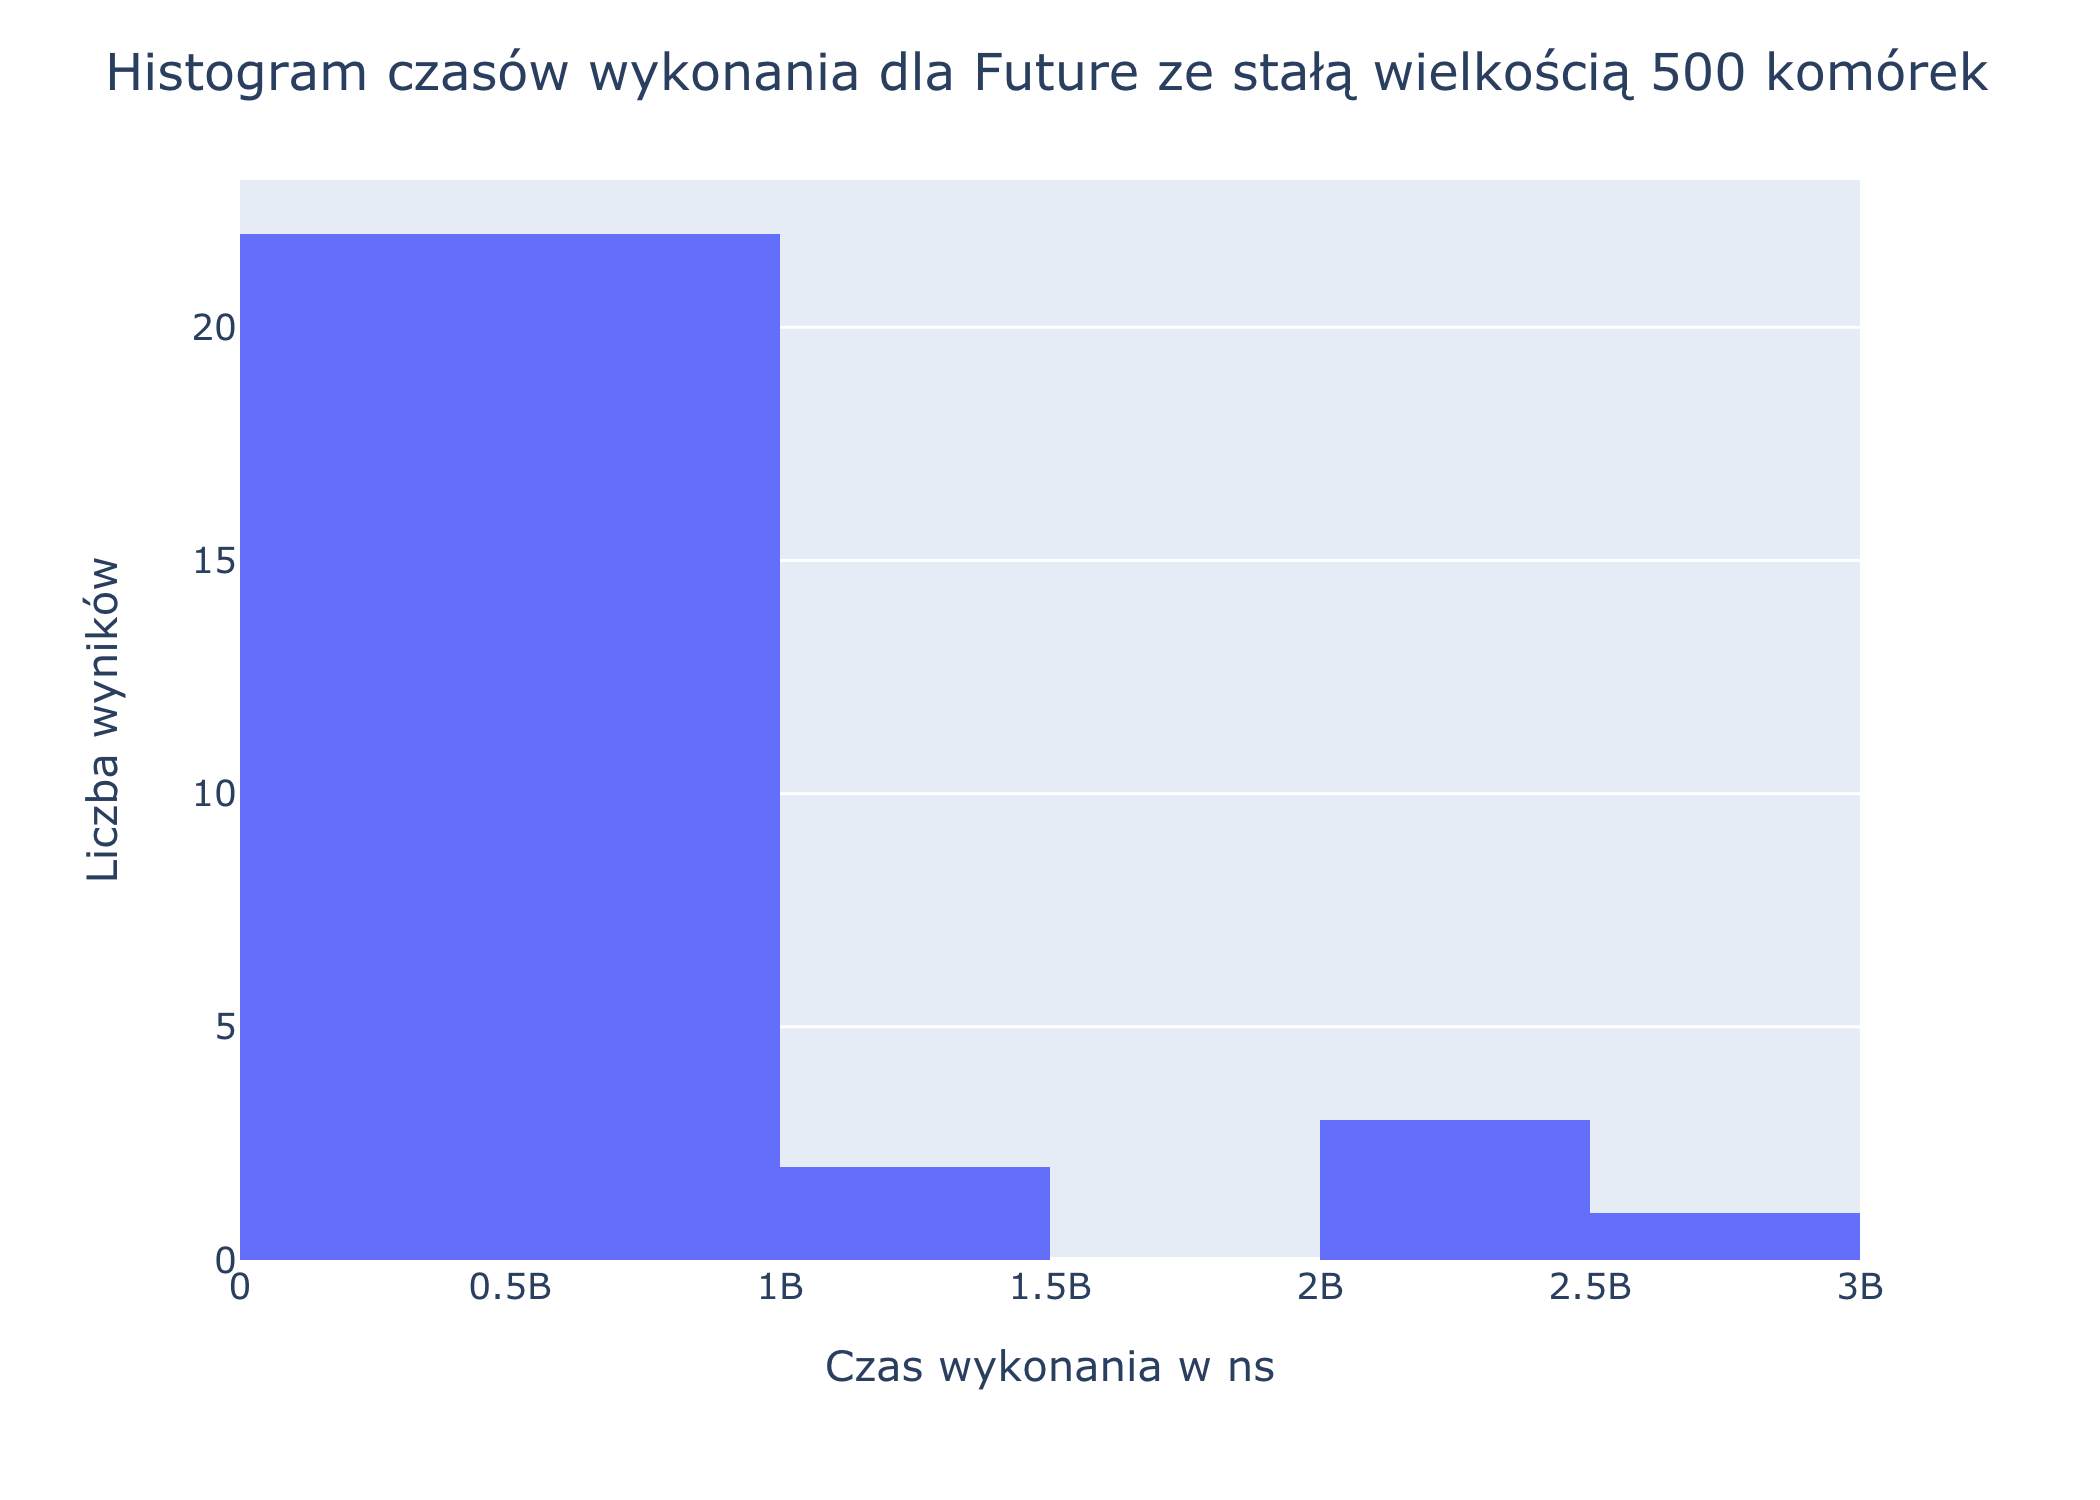
\includegraphics[width=0.9\textwidth]{Parallel_Future_fix_chunk_500_game_of_life_performance}
  \caption{Histogram czasów wykonania dla Future ze stałą wielkością 500 komórek}
\end{figure}

\subsubsection{Liczba Future równa ilości rdzeni}
\paragraph{Średni czas symulacji: } 1073.90 ms


\begin{figure}[H]
  \centering
  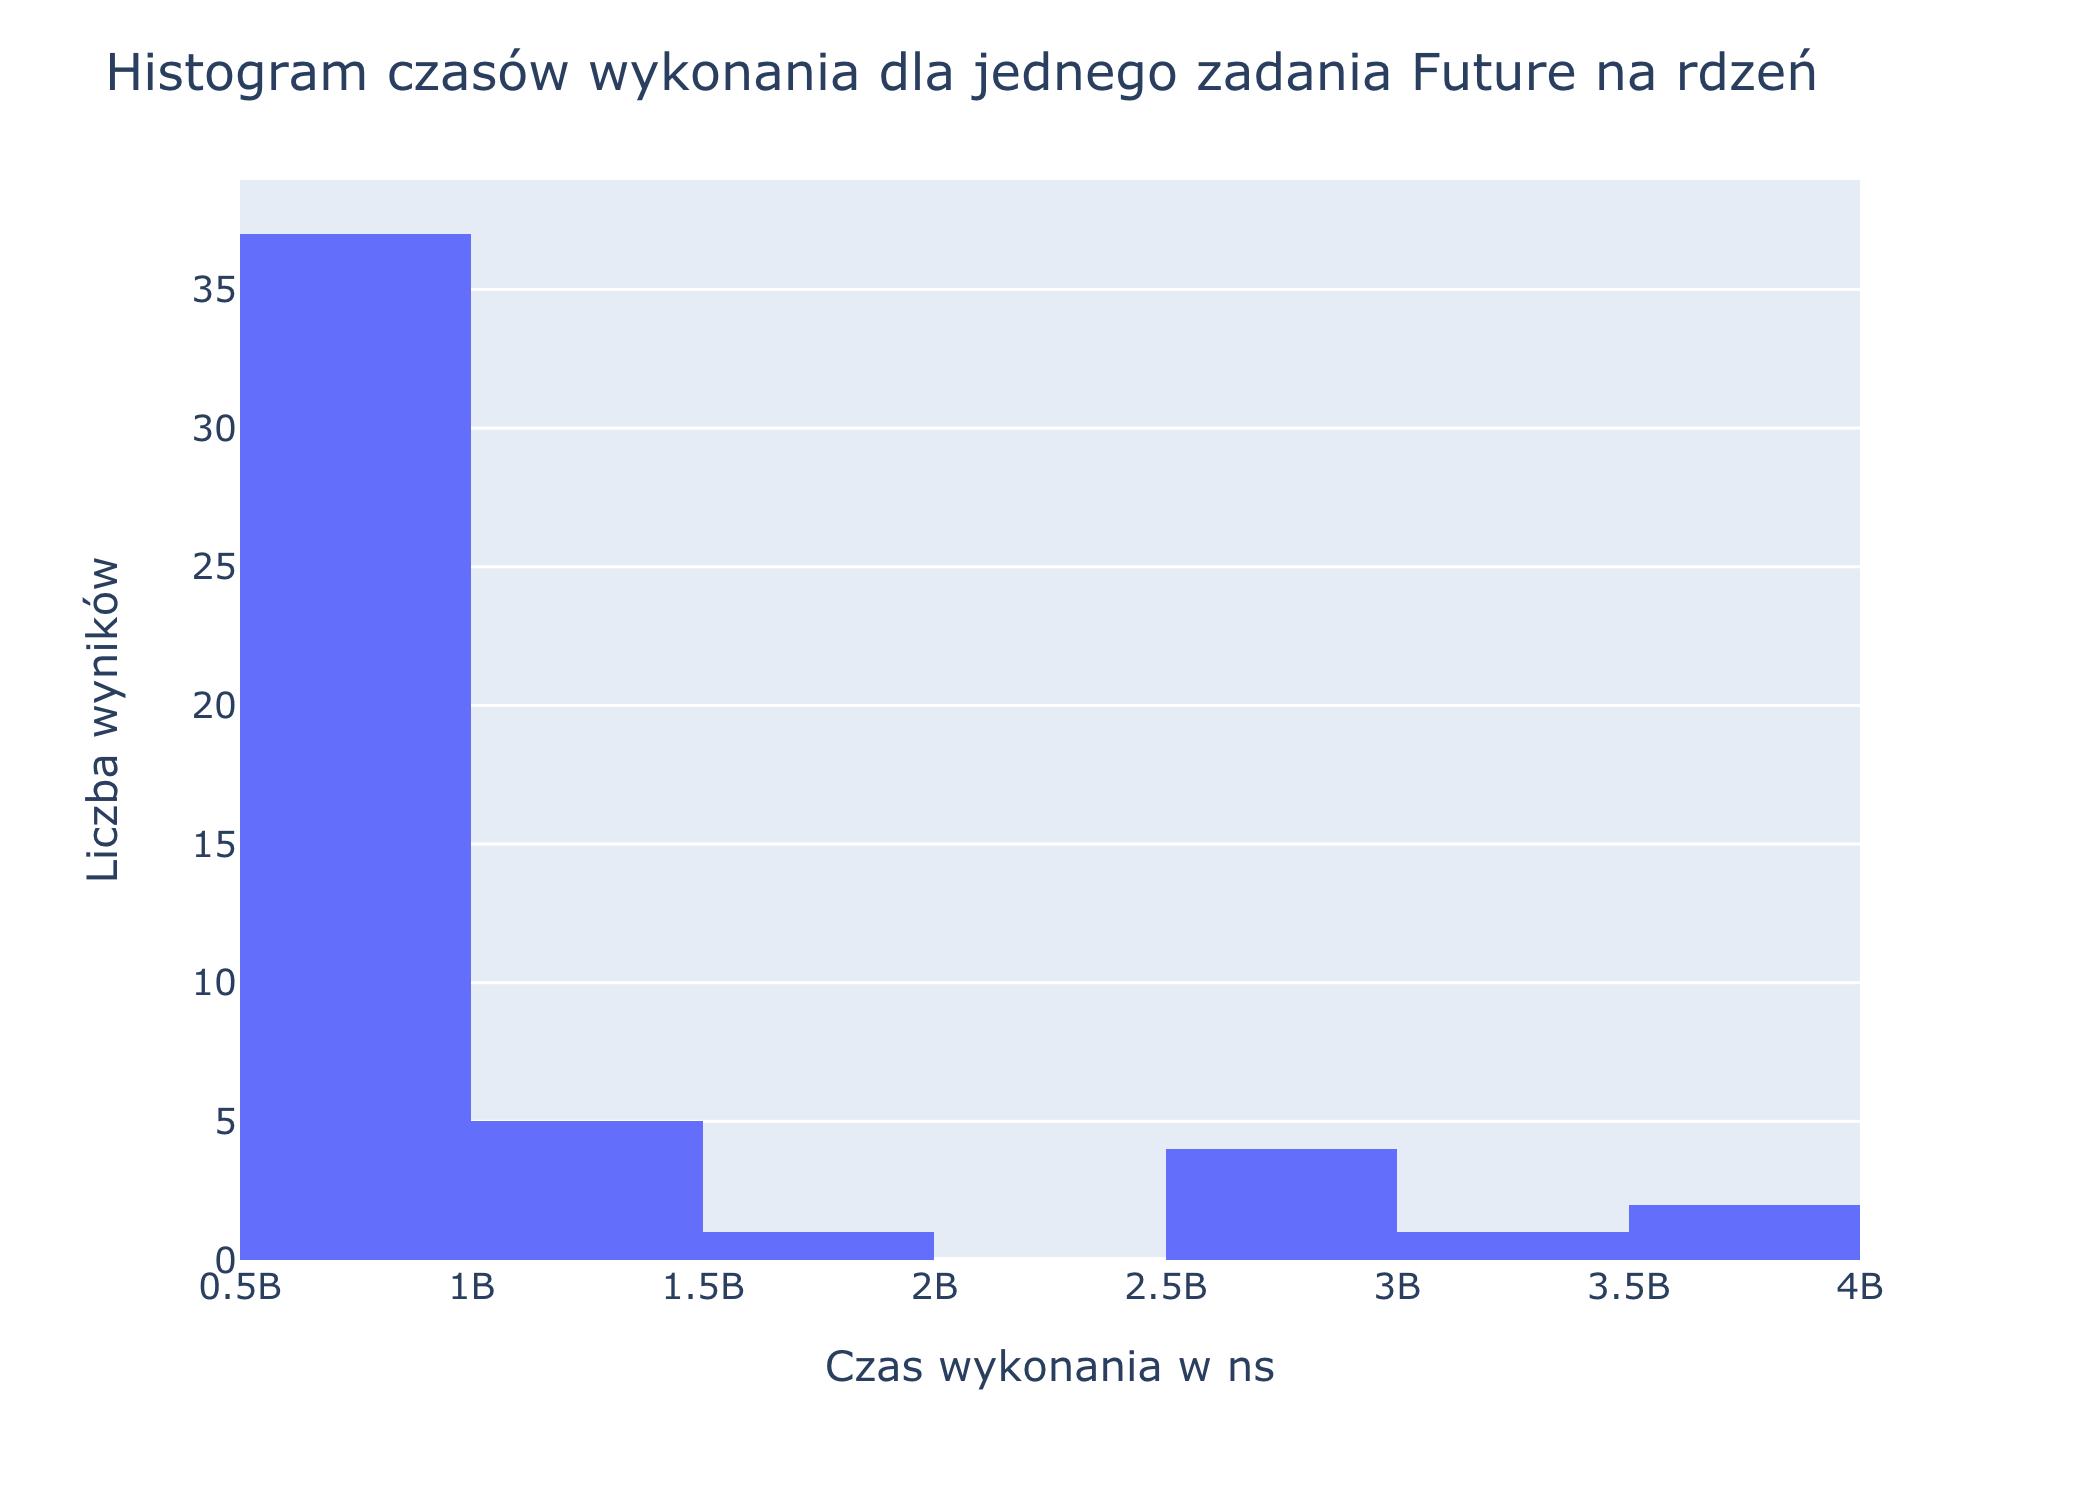
\includegraphics[width=0.9\textwidth]{Parallel_Future_One_For_Each_Thread_of_life_performance}
  \caption{Histogram czasów wykonania dla jednego zadania Future na rdzeń}
\end{figure}

\subsection{Thread API}
Zbadanie wydajności programu przy zastosowaniu klas \texttt{Runnable} i \texttt{Thread}.

\subsubsection{Thread ze stałą wielkością komórek}
Uruchomienie tylu wątków, żeby każdy miał wielkość zadania 200.
\paragraph{Średni czas symulacji: } 14191.27 ms


\begin{figure}[H]
  \centering
  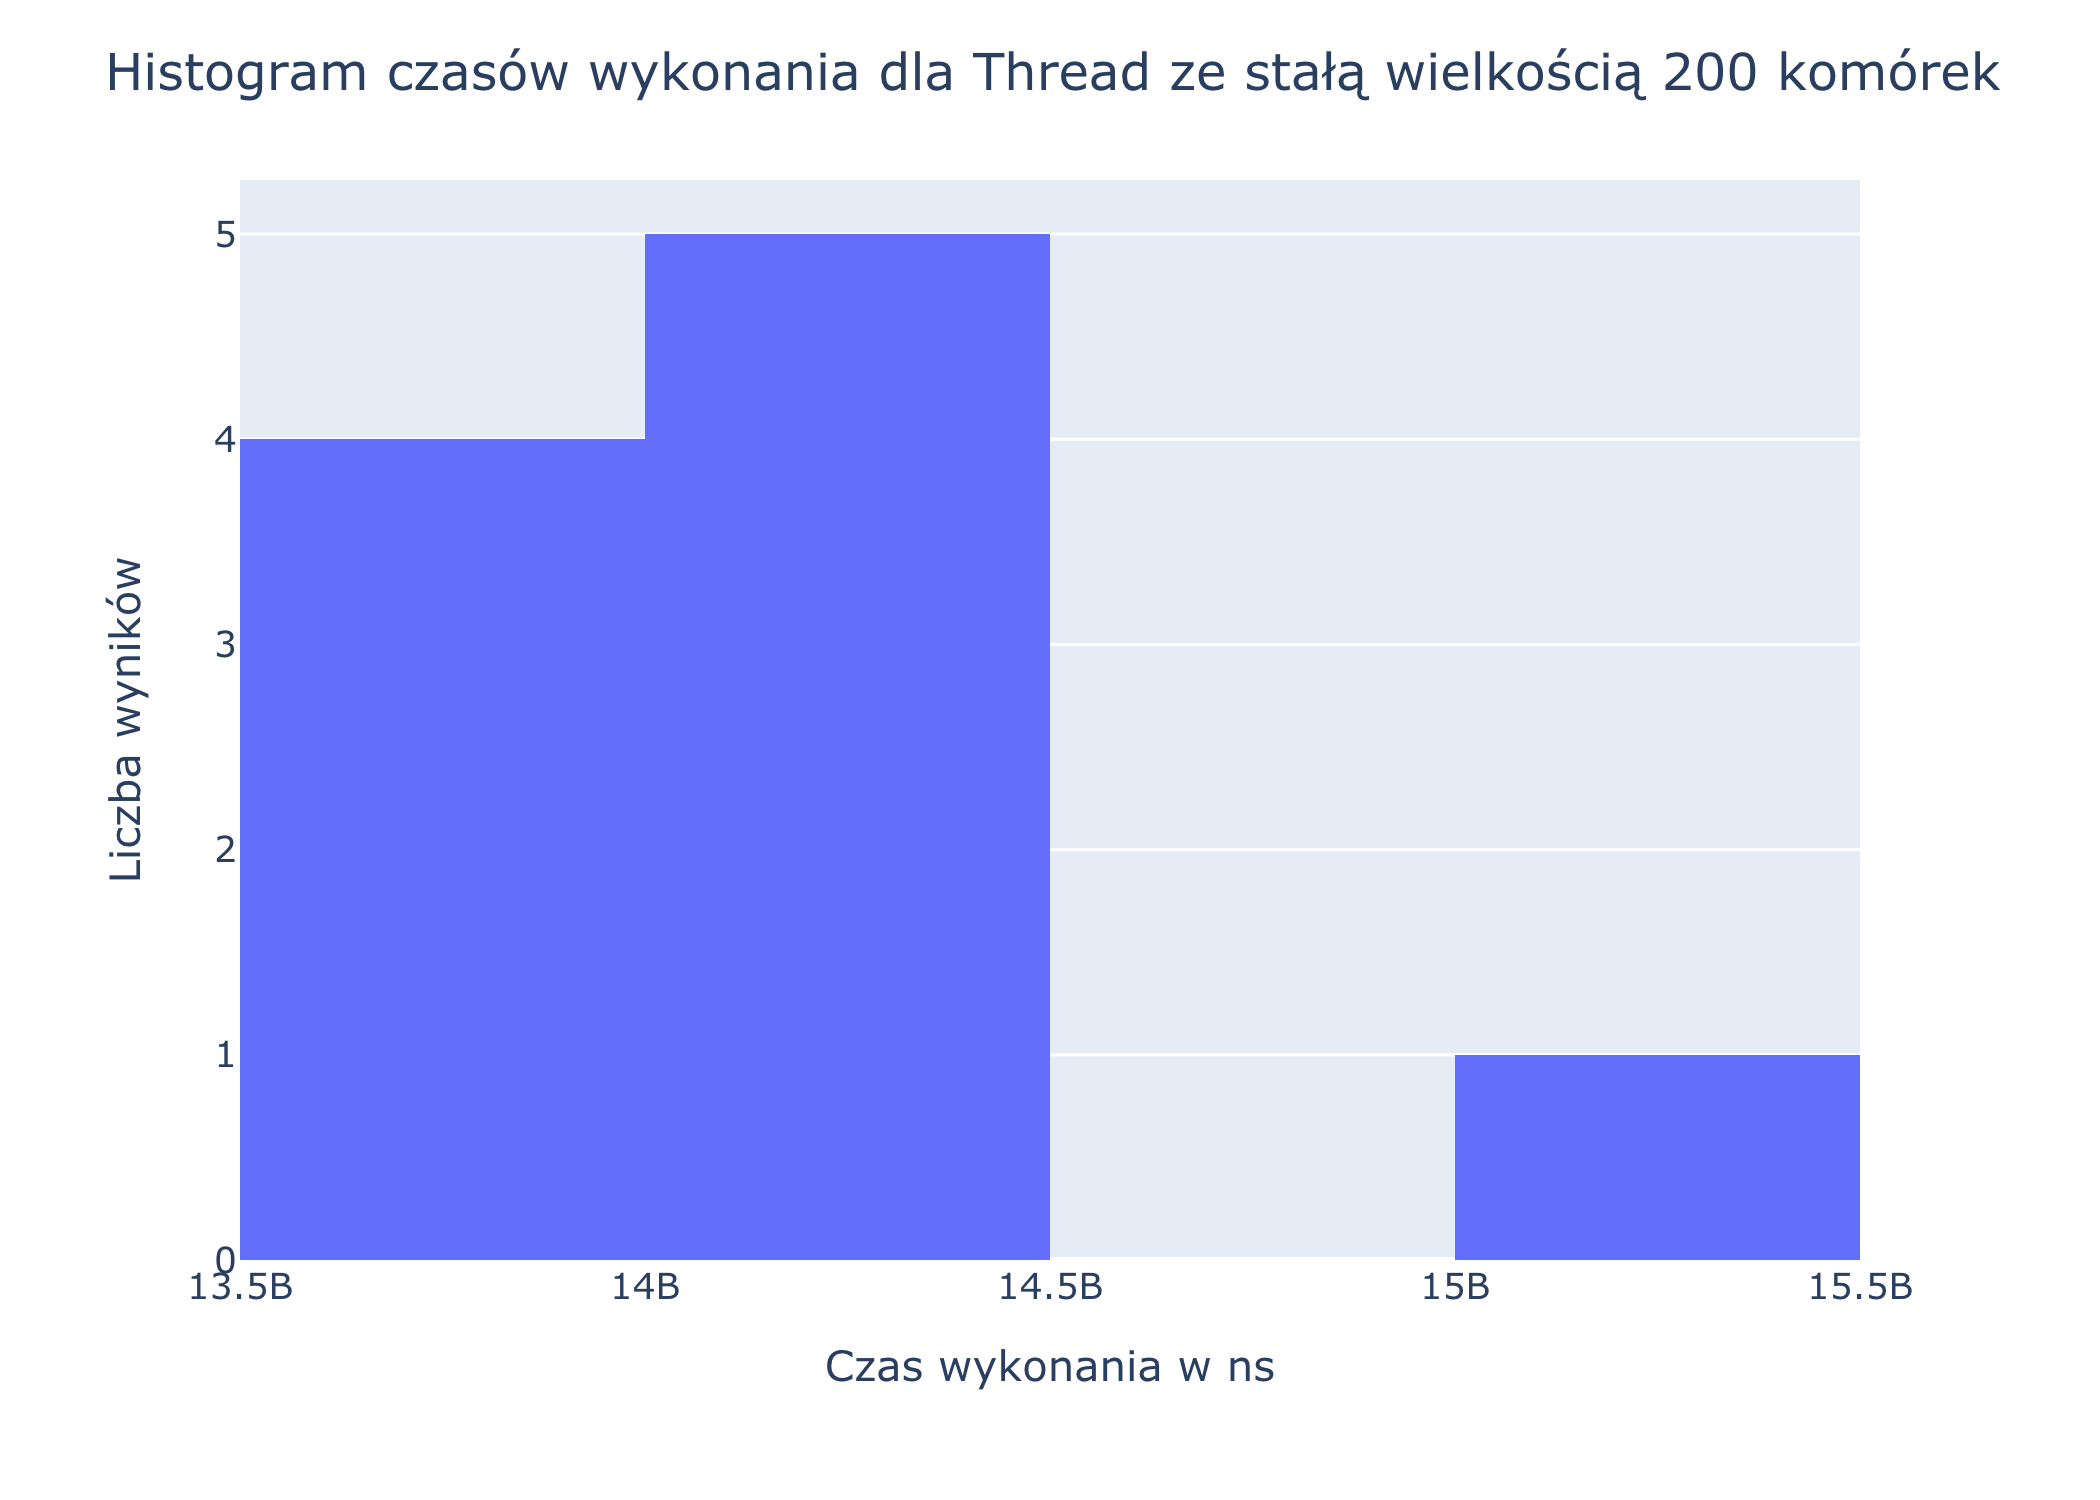
\includegraphics[width=0.9\textwidth]{Parallel_Thread_fix_chunk_200_game_of_life_performance}
  \caption{'Histogram czasów wykonania dla Thread ze stałą wielkością 200 komórek'}
\end{figure}

\subsubsection{Liczba Thread równa ilości rdzeni}
\paragraph{Średni czas symulacji: } 866.45 ms


\begin{figure}[H]
  \centering
  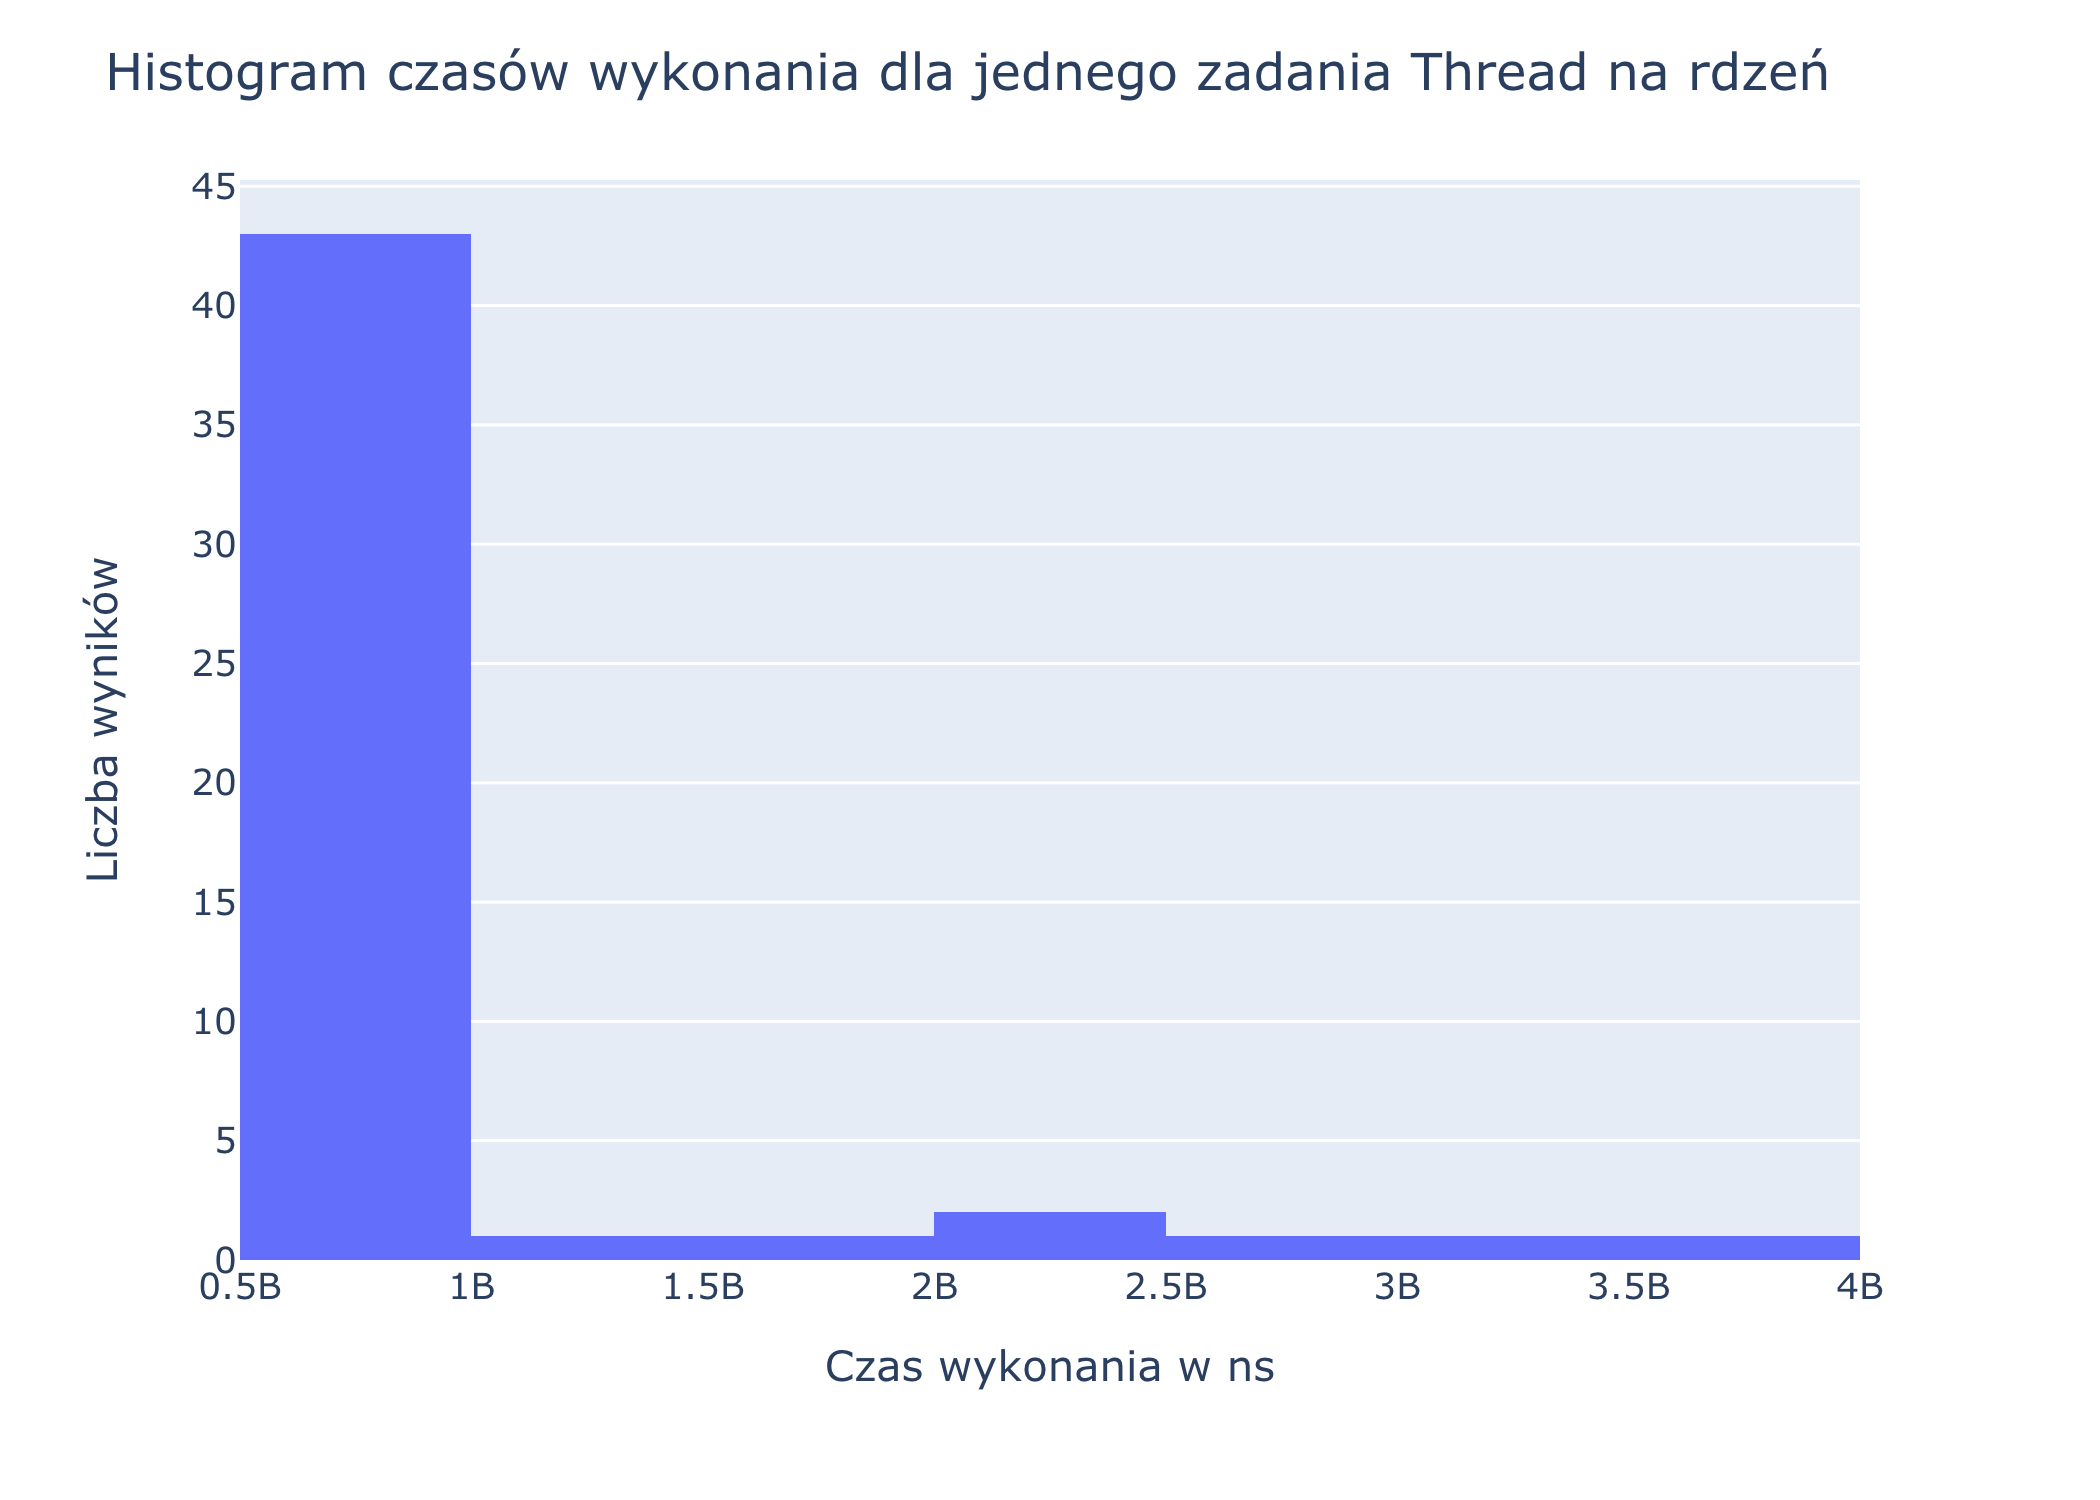
\includegraphics[width=0.9\textwidth]{Parallel_Thread_One_For_Each_Thread_of_life_performance}
  \caption{Histogram czasów wykonania dla jednego zadania Thread na rdzeń}
\end{figure}

\subsection{Porównanie wyników}
Zestawienie średnich czasów obliczeń uzyskanych dla różnych podejść.

\begin{figure}[H]
  \centering
  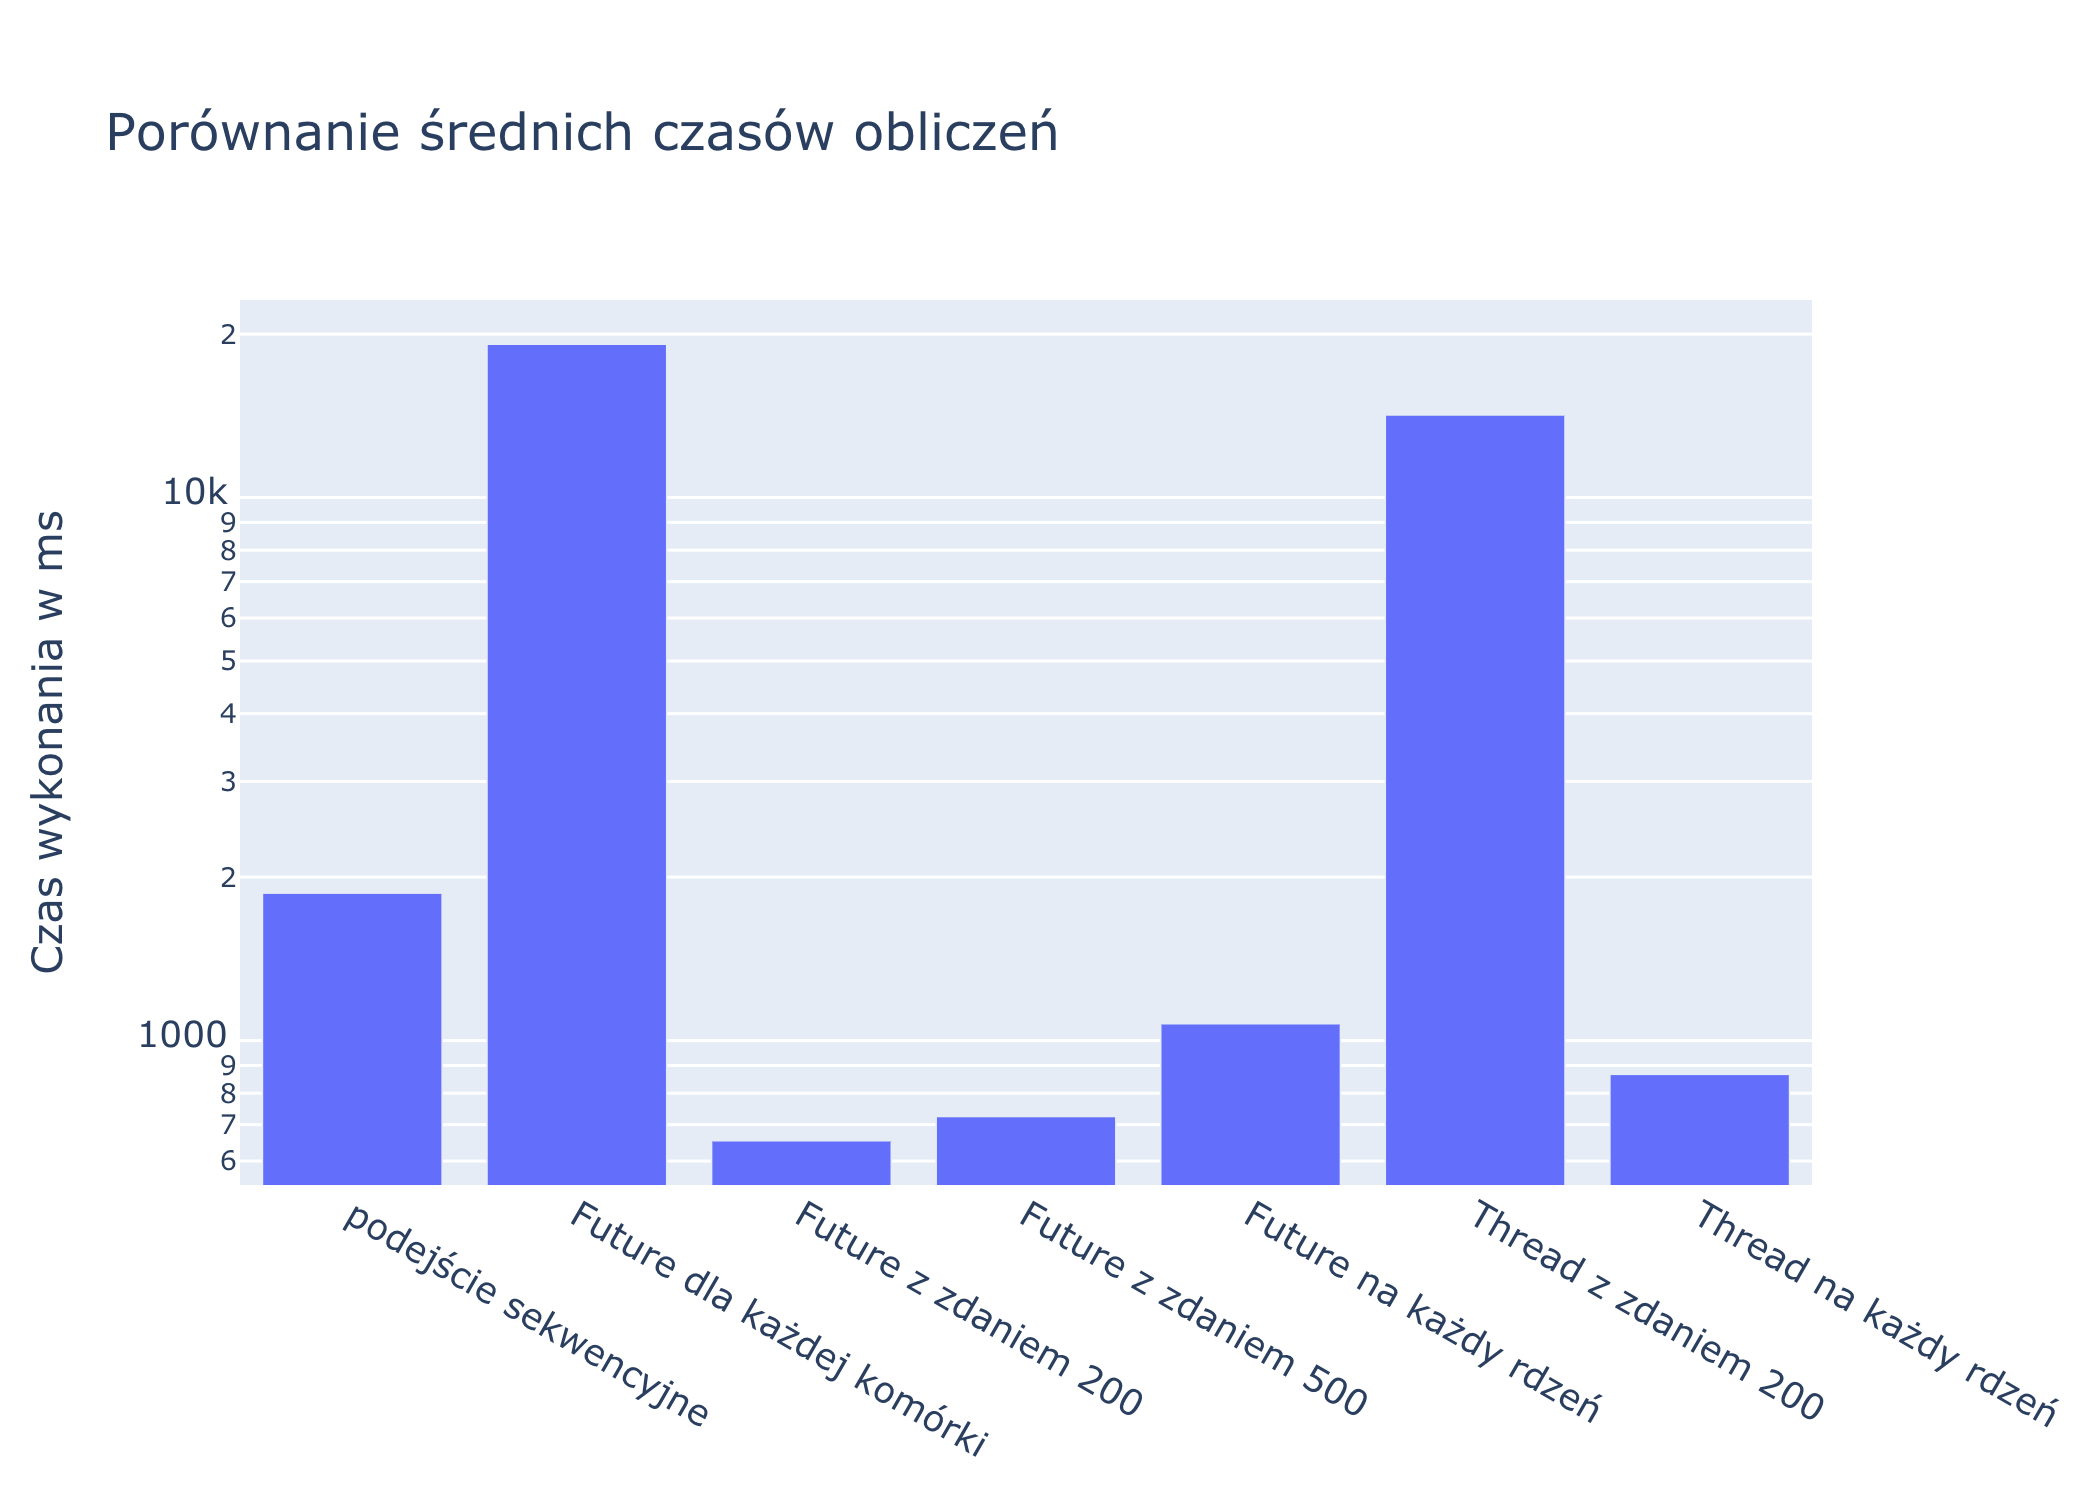
\includegraphics[width=0.9\textwidth]{Result_comparasion}
  \caption{Porównanie średnich czasów obliczeń}
\end{figure}


\section{Wnioski}

Zastosowanie obliczeń równoległych pozwala na uzyskanie znacznego przyśpieszenia jednak wymaga odpowiedniej realizacji. Przy zastosowaniu nieodpowiedniego podejścia czas wykonania może zostać znacząco wydłużony. Przykładem może być podejście z zachowaniem maksymalnej ziarnistości, które wypadło najgorzej. Prawdopodobnie duże opóźnienie stanowi wtedy tworzenie oraz obsługa tak ogromnej liczby klas \texttt{Future}.

Równie słaby wynik dało podejście z zastosowaniem wątków o stałej wielkości zadania. Ponieważ wielkość zdania była mała w stosunku do wielkości problemu powstało bardzo dużo wątków. Prawdopodobnie spory narzut stanowiło wywłaszczanie wątków i przełączanie między nimi.

Podejście z ilością obiektów \texttt{Future} równą liczbie rdzeni wypadło trochę gorzej niż dla liczby wątków równej liczbie rdzeni. Świadczy to o narzutach płynących z abstrakcji stosowanych w \textit{Concurrency API}.

Najlepszym rozwiązaniem okazało się zastosowanie obiektów \texttt{Future} ze stałą wielkością zadania. W przeciwieństwie do analogicznego schematu z wątkami dla \texttt{Future} nie powstała nadmiarowa liczba wątków procesora. Takie podejście prawdopodobnie pozwoliło zniwelować opóznienie płynące z różnego tempa pracy poszczególnych rdzenie dzięki rozłożeniu pracy metodą przypominającą technikę \textit{load balancing}.

\vspace{5mm}

\textit{Concurrency API} pozwala na łatwe zarządzanie grupą wątków. Wymaga jednak zaplanowania sposobu korzystania z \texttt{ExecutorServices}. Dzięki dodatkowej warstwie abstrakcji praca w tym schemacie jest przyjemna. Jednak takie podejście uniemożliwia zastosowania zaawansowanych technik programowania równoległego.

\vspace{5mm}

Zastosowanie testów jednostkowych w projekcie znacznie ułatwiła wprowadzane zmian w kodzie. Dzięki ich obecności wykrycie błędów oraz sprawdzenie czy symulacja jest wykonywana poprawnie było szybkie. Pozwoliło to na swobodne testowanie różnych rozwiązań.

\end{document}
